\documentclass{article}
\usepackage[utf8]{inputenc}
\usepackage[margin=2.6cm]{geometry}
\usepackage{float}
\usepackage{rotating}
\usepackage{graphicx}
\usepackage{caption}
\usepackage{subcaption}
\usepackage[round]{natbib}
\usepackage{setspace}
\usepackage{longtable}
\usepackage{lscape}
\onehalfspacing
\usepackage{tikz}
\usetikzlibrary{arrows,automata,positioning,shapes}
\usepackage{adjustbox}
\usepackage{amsmath}
\usepackage{tabularx}
\usepackage{multirow}

\title{The role of individual resource dynamics in the variability of life cycles in a female human population.
\\
Registered Report}
\author{Pablo J. Varas Enriquez, Monique Borgerhoff Mulder, Heidi Colleran, Dieter Lukas*\\\\
* No special order of authors}
\date{\today}

\begin{document}

\maketitle

\tableofcontents

\begin{abstract}
    The female human life cycle is characterized by a long lifespan, within which there is usually a short reproductive period in between long juvenile and post-reproductive stages. Within those boundaries, there is a high variability in the length of longevity, and the timing and outcome of reproduction, usually associated with a life history trade-off between survival and fertility. The evolution of the female human life cycle has been related to the surplus of resource production during adulthood and the inter-generational transfers towards juveniles. However, there is no clear understanding whether and how these resource dynamics shape the observed variation within human populations. Here we develop a theoretical framework to describe how different resource dynamics influence the variability of the female human life cycle. For this, an agent-based model is used to structure and describe how resource dynamics (i.e. production, consumption, sharing, and storage) at different developmental stages of individuals can lead to different variability levels within a population. Furthermore, the model is set under multiple combinations of production and sharing probabilities (i.e. high, medium, and low), as well as habitat qualities (i.e. high and low) in order to assess how production and sharing play different roles in the variability of life cycles among individuals. We expect that differences in the ways in which individuals obtain and allocate resources across their lifespan can contribute to understand the boundaries under which the female human life cycle varies, allowing to understand other possible scenarios beyond the common longevity versus fertility trade-off. 
\end{abstract}

\section{Introduction}

There are many paths an individual can follow through its life cycle, which is the basis of the diversity seen across the tree of life. The diversity of mortality schedules can lead to lifespans that vary from days to thousands of years (e.g. hairyback vs patagonian cypress \citep{balsamo1988life,lara19933620}) and reproductive outputs can go from a couple to thousands of offspring (e.g. eastern hemlock vs rain moth \citep{tindale1932revision,van2017lifetime}. Within the tree of life, the female human life cycle is characterized by a long lifespan and a short reproductive career, framed within long juvenile and post-reproductive stages \citep{kaplan2000theory}. Within these boundaries, the life cycle of female humans also varies in terms of mortality and fertility. Populations can differ in their average life expectancy by a factor of 2 and their average reproductive output by a factor of 5 (e.g. foraging populations \citep{migliano2007life} versus post-demographic transition populations \citep{de2017maximum}). The diversity of life cycles observed among female human populations is fuelled by the differences in longevity and fertility between individuals within a population. For example, xx\% of female individuals are childless in a population with high fertility rates. However, it is not clear if the within-population variability of female human life cycles is explained by the same processes that explain the differences among species across the tree of life. 

The differences in life cycles among species have usually been related to the trade-offs in which an individual allocates the limited resources available in its environment towards life history traits such as survival or reproduction \citep{stearns2000life}. The fast-slow continuum is a key life history framework to explain differences at the species level, where some species show a ``fast" strategy by having a short lifespan but a high reproductive output whereas those with a ``slow" strategy live longer but reproduce less \citep{stearns1983influence}. However, further analyses have shown that life history strategies among species have more than one dimension, showing that reproductive strategies \citep{salguero2016fast}, the distribution of mortality risk \citep{healy2019animal}, and individual stochasticity of life history traits \citep{varas2022individual} play major roles in the explanation behind the diversity of life cycles across the tree of life. Hence, the multiple ways in which individuals within a population trade-off the allocation of resources have lead to the evolution of a high diversity of life cycles among populations and species.

The diversity seen among species and populations is fuelled by the variability of life cycles at the individual-level. Evolutionary models that focus on the differences in longevity and reproduction among individuals have been developed in terms of adaptive developmental plasticity and the balance between resource acquisition and allocation. Adaptive developmental plasticity is the capacity of an individual to produce different phenotypic outcomes depending on environmental inputs during the development of the individual \citep{stearns1989evolutionary}. Here, the individuals who develop a phenotype in response to the inputs they receive early in life should be the ones with a higher fitness than their counterparts, whereas those who do not experience the early-life inputs and do not develop the phenotype show a higher fitness than those who develop the phenotype without early-life inputs \citep{bateson2004developmental}. Furthermore, there are two types of models: the informational model, where the early-life input provides information about the future environment, and the somatic state-based model, where the input alters the somatic state of the individual, indirectly developing the phenotype associated with higher fitness \citep{nettle2015adaptive}. On the other hand, the work relating resource acquisition and allocation is mainly based on the work of \cite{van1986acquisition}. Here, they show that with high variability of resource acquisition comes a low variability of resource allocation towards reproduction, which makes that individuals who live longer also have the highest reproductive output within a population (i.e. phenotypic masking). Recent reviews on their model from the pace-of-life syndrome framework show that resource acquisition plays an equal, or bigger, role than resource allocation to understand the differences in survival and reproduction among individuals, phenotypes, and within individuals \citep{laskowski2021integrating,haave2022differences}. However, neither of the approaches consider the social basis that comes with resource transfers among individuals, which diversify the ways in which resources or inputs are acquired and distributed.    

In the case of humans, the differences in longevity at an individual level have been associated with resource availability (i.e. more resources equals longer lifespans) \citep{kaplan2003embodied}, while the relationship of fertility with resources is more complex \citep{mulder1998demographic,sear2016understanding}. Sharing dynamics have also been proposed as a key component to understand the different life cycles among female humans, due to the social nature of our species. Here, the presence of different members of the population have been associated with differences in the longevity and reproductive output of female individuals, as can be found in the literature related to cooperative breeding, sibling competition, female conflict, among others \citep{ivey2000cooperative,nitsch2013elder,mace2012female,sear2011much}. However, research in the area usually focus on specific life history traits of the life cycle (e.g. longevity, number of descendants) rather than addressing them together, and/or specific ways in which resources are available for female individuals (e.g. amount of food, presence of the grandmother). Therefore, the understanding of the mechanisms linking the variability of life cycles within a female human population with resource availability remains limited.

Models that address the limitations of how the life cycles of women in a population are shaped by resource availability focus on the conditions that differentiate the female human life cycle from other species. The ``embodied capital model" suggests that the surplus of resource production during adulthood allows the evolution of the female human life cycle \citep{kaplan2000theory}. This model proposes that the difference between resource production and consumption allows high parental investment, translated in short interbirth intervals and long post-reproductive periods for the parents and long juvenile periods for their offspring. The ``pooled energy model" deepens in this framework by suggesting that alloparenting from individuals of different generations would allow to decrease the load of parental investment \citep{kramer2010pooled}. The ``inter-generational resource transfer model" poses that inter-generational transfers would play a major role in the mortality and fertility schedules of human populations. As developed by \cite{lee2003rethinking}, this model suggests that age-specific mortality is proportional to the remaining reproductive value and resource transfers made at later ages, predicting the early-life and later-life mortality patterns characteristics of the female human life cycle. Additionally, Chu and Lee further develop the ``inter-generational resource transfer model", showing that transfers co-evolve with low mortality, since adults are more efficient to produce energy, which is transferred to juveniles, who are more efficient to turn that energy into body size, allowing lower mortality \citep{chu2006co}. While these models show that the female human life cycles co-evolved with the interplay of resource acquisition and transfers, they do not address how different resource dynamics can shape the variations of the life cycle within a population.

Our aim is to develop a theoretical framework to understand how resource dynamics (i.e. resource production, transfers, and storage) and habitat quality influence individual-level variations of the female human life cycle. The model would focus on how the variability of life cycles within a female human population changes due to stochastic differences in resource production, transfer, and storage under poor and rich environments (see a summary in Table \ref{tab:1}). The framework will be developed with an agent-based model, because of its capacity to address complex phenomena from individual and population levels, as well as address stochasticity among individuals by allowing agents to behave differently despite being all under the same rules \citep{judson1994rise,wilensky2015introduction}. This last attribute of agent-based models is interesting for our purposes, because resource dynamics are understood as variables that play a role in the boundaries of variability of life cycles at an individual and population level. The model will be described using an ODD (Overview, Design concepts, Details) protocol, as an standardised way to clarify the scope, assumptions, and parameters used to answer our questions \citep{grimm2006standard,grimm2020odd}.

\section{Model description}

\subsection{Purpose and patterns}

The purpose of the model is to understand how different resource dynamics and environments influence the variations of the female life cycles within a population. The mechanism expected to influence the life cycle at an individual level is in the interplay of resource production and transfer which allows individuals to allocate resources to survival, life stage transitions, and reproductive timing and output. Variability of the female human life cycle at the population level would be explained by the distribution of different life cycles that arise from individual differences, which are based on the mechanism described earlier. The expected patterns can be described based on the resource dynamics and habitat quality. First, the life cycles among individuals should vary more due to differences in the amount of resources produced across the life cycle than because of resource transfers or storage. This pattern would be because transfers and storing dynamics would play a buffering role, by compensating the surplus and/or lack of resources that can be allocated in the components of the life cycle. Second, the patterns of resource dynamics should also vary depending on the amount of resources individuals can get from their environment (i.e. habitat quality), expecting that the variability of life cycles decreases as habitats have a higher quality (see Table \ref{tab:1} and \ref{tab:2} for a summary).
\\\\
The life cycle of a female individual will be described by the time spent across four discrete stages (i.e. juvenile, adult, reproductive-career, post-reproductive), which are defined by the timing of key events of the life course (i.e. age at menarche, age at first reproduction, and age at menopause). Longevity will also be a characteristic of the life cycle (i.e. number of years alive), as well as lifetime reproductive output (i.e. number of descendants through life). The influence of resource dynamics into the life cycle will be understood by the timing of reproductive events (i.e. age at first and last reproduction, and average interbirth intervals) and life stage transitions (i.e. age at menarche, age at first reproduction, age at menopause), as well as longevity and lifetime reproductive output. Finally, resource dynamics will be characterized by the amount of resources produced, transferred, and stored throughout the life cycle. Consumption is understood as the amount of resources used to cover survival and reproductive costs. A graphical representation can be seen in Fig. \ref{fig:1}. Finally, there will be different scenarios based on combinations of probabilities of resource production and sharing (i.e. high, medium, low) as well as habitat quality (i.e. high, low) (see Table \ref{tab:2} for a summary).

\subsection{Entities, state variables, and scale}

\subsubsection{Entities}

Individuals represent females in a single-sex population. A single-sex population is used because the model is focused on the female human life cycle, under the assumption that it evolves independently from the male counterpart. Individuals that are born until they reach age of menarche are considered juveniles. Adults are individuals that have reached menarche until they have their first descendant or reach menopause. Adults transition to a reproductive-career stage once they have their first reproduction, and remain in this stage until they reach menopause. From menopause onward individuals are considered post-reproductive.

\subsubsection{State variables}

Every individual in the simulation is characterised by state variables that are a) calculated new in each iteration, and b) modified from one iteration to the next.

Variables that are calculated new in each iteration:
    \begin{itemize}
        \item Production: Individual production of resources by the individual. Whether an individual produces resources (1) or not (0) is based on a Bernoulli distribution with a stage-specific probability. Also, the amount of resources that are produced is fixed to each life cycle stage. Production can be defined as:
\begin{equation}
    y_{i,t}=\begin{cases}
    y_s,& \text{Bernoulli}(P_s)=1\\
    0,& \text{Bernoulli}(P_s)=0
\end{cases}
\end{equation}
        Where $y_{i,t}$ is the amount of resources produced by individual $i$ at time $t$, $y_{s}$ the amount of resources that can be produced at stage $s$, and $P_{s}$ the probability of resource production at stage $s$.
        \item Maternal investment: An individual would transfer under a need-based dynamic her stored resources from the previous iteration or the ones produced in the current one to the descendants that do not have enough resources to cover their survival effort.
        \item Number of transfers: the number of transfers an individual would give away or receive resources would be determined by a stochastic block model, where the number of ties an individual has is randomly determined by the surplus of resources available.
        \item Resource transferred: The amount of resource that an individual transfers among her ties is the surplus of production divided by the number of ties she has:
\begin{equation}
    rt_{i,t}=\frac{y_{i,t}-p_e+m_e}{number of ties}        
\end{equation}
        Where $rt_{i,t}$ is the amount of resource transferred by individual $i$ at time $t$, $y_{i,t}$ is the amount of resources produced, $p_e$ is survival effort, $m_e$ is reproductive effort, and $number of ties$ is the number of ties the individual has.
        \item Resource received: The amount of resource received by an individual is the sum of the resources transferred to her from the ties she formed in ``Number of transfers":
\begin{equation}
    trr_{i,t}=\sum_0^j rr_j        
\end{equation}
        Where $trr_{i,t}$ is the total amount of resources received by individual $i$ at time $t$, and $rr_j$ is the amount of resource received by individual $j$.
        \item Resources available: The amount of resources available after the resource dynamics of production and transfers, that will be used by the individual to cover the costs of survival, reproduction, and transition.
\begin{equation}
    ra_{i,t}=w_{i,t-1}+y_{i,t}-mi_{i,t}-rt_{i,t}+trr_{i,t}        
\end{equation}
        where $ra_{i,t}$ is the amount of resources available for individual $i$ at time $t$, $w_{i,t-1}$ the stored resources from the previous iteration, $y_{i,t}$ the amount of resources produced, $rt_{i,t}$ and $trr_{i,t}$ the resources shared, and $mi_{i,t}$ the maternal investment in the current iteration.
        \item Survival: Whether the individual survives (1) or not (0) in the iteration, which depends if the individual has enough resources available. The survival is defined as:
\begin{equation}
    p_i=\begin{cases}
    1,& ra_{i,t} \geq pc\\
    0,& ra_{i,t} < pc
\end{cases}
\end{equation}
        Where $p_i$ is the survival output of individual $i$, $ra_{i,t}$ is the amount of resourced available by individual $i$ from the previous iteration ($t-1$), and $pc$ is the survival cost.
        \item Reproduction: Whether the female individual reproduces (1) or not (0) in the iteration, which depends if she has enough resources stored to cover the reproductive costs. Reproduction is defined as:
\begin{equation}
    m_i=\begin{cases}
    1,& w_{i,t} \geq mc\\
    0,& w_{i,t} < mc
\end{cases}
\end{equation}
        Where $m_i$ is the reproductive output of individual $i$, $w_{i,t}$ is the amount of resourced stored by individual $i$ at time $t$. $mc$ is the reproductive cost.
        \item Transition: Whether a female individual transitions (1) or not (0) to the next life cycle stage, which depends if she has enough resources available to allocate towards the key event of transition.
\begin{equation}
    t_i=\begin{cases}
    1,& ra_{i,t} \geq tc\\
    0,& ra_{i,t} < tc
\end{cases}
\end{equation}
        Where $t_i$ is the transition output of individual $i$, $ra_{i,t}$ is the amount of resources available, and $tc$ is the key event of transition. The transitions are defined as follow:
        \begin{itemize}
            \item Age at sexual maturity: A juvenile female individual reaches menarche once she has enough resources to cover the costs of survival and ten times the reproductive costs.
            \item Age at first reproduction: An individual in the adult stage has her first descendant once she has enough resources to cover the survival and reproductive costs.
            \item Age at menopause: A female individual reaches menopause once she has enough resources to cover the survival costs but has not covered the costs for reproduction in the last 20 iterations. 
        \end{itemize}
\begin{equation}
    tc=\begin{cases}
    ASM_i,& ra_{i,t} \geq pc+10mc\\
    AFR_i,& ra_{i,t} \geq pc+mc\\
    AM_i,& pc \geq ra_{i,t} < mc_{i,t-20...t}
\end{cases}
\end{equation}
        Where $T_i$ is the function for life cycle transition of individual $i$, $ASM$ is age at sexual maturity, $AFR$ is age at first reproduction, and $AM$ is age at menopause of individual $i$.
    \end{itemize}
Variables that are modified from one iteration to the next:
    \begin{itemize}
        \item Age: Amount of iterations the individual goes through from its birth until it dies. Age increases by one after each iteration, reflecting one year.
        \item Lifetime reproductive output: Amount of descendants produced. Reproductive output increases by one after an iteration, if reproductive requirements are met.
        \item Stage: Life cycle stage in which the individual is at the moment. There are four stages (juvenile, adult, reproductive-career, post-reproductive), each with its own stage-specific resource dynamics. 
        \item Resources stored: Amount of resources the individual stores for later in time (i.e. next iteration). The amount of resources stored depends on the surplus resources after the stage-specific resource and life-history dynamics. Resources stored is defined as:
\begin{equation}
    w_{i,t}=ra_{i,t} - pe - me - tc
\end{equation}
    Where $w_{i,t}$ is the amount of stored resources of individual $i$ at time $t$, $ra_{i,t}$ is the amount of stored resources of individual $i$ at time $t-1$, $pe$ is survival effort, $y_{i,t}$ is the amount of resources produced by individual $i$ at time $t$, $R_{i,t}$ is the amount of resources received by individual $i$ at time $t$, $G_{i,t}$ is the amount of resources gave away by individual $i$ at time $t$, and $me$ is reproductive effort.
    \end{itemize}

\subsubsection{Auxiliary variables}

The individual dynamics are constrained by the following auxiliary variables. These variables are stage-specific, set at the initialisation and apply to all individuals.

\begin{itemize}
    \item Survival cost: Amount of resources necessary to cover the costs of survival.
    \item Reproductive cost: Amount of resources necessary to cover the costs of reproduction.
    \item Number of descendants per reproduction: A female individual produce only one descendant per reproductive event.
    \item Produce: Probability of producing resources ($P_s$) that is used in the state variable ``Production".
    \item Habitat quality: Amount of resources an individual can produce in the iteration.
    \item Receive: Probability of receiving resources from another individual(s). The probability is based on a distribution starting in zero and a maximum value based on \cite{gurven2004give}.
    \item Give: Probability of giving resources to another individual(s). The probability is based on a distribution starting in zero and a maximum value based on \cite{gurven2004give}.
\end{itemize}

\subsubsection{Scale}

Each iteration in the model represents one year. The probability  of producing is Bernoulli, with the values of happening ($1$) or not ($0$). The times that resources are received or gave away can be a minimum of zero (i.e. no receiving/giving) and a maximum based on the surplus of resources available and the dynamics set in the stochastic block model. The amount of resources and probability that an individual produces, receives, and gives are stage-specific. Survival and reproductive effort are evaluated after the resource dynamics, followed by the evaluation for stage transition. Finally, the amount or resources available are stored and passed from one year to the next.

\subsection{Process overview and scheduling}

Every dynamic described in the following process is stage-specific. In the juvenile stage, individuals go through the produce, sharing, and survive models each year until they reach sexual maturity, transitioning to the adult stage. In the adult stage, individuals go through produce, sharing, and survive models until they have their first descendant or reach menopause. If an adult transitions to a reproductive-career stage, she goes through produce and sharing models followed by reproduction and survive models until she reaches menopause. Once in a post-reproductive stage, the individual goes through the produce, sharing, and survive models of the stage. In each year, the individual increase her age and updates the amount of resources she stores. During each transition, the individual updates her stage variable and also transitions with the resources she has stored from the earlier stage.
\\\\
The scheduling of the process starts with the production model, followed by the maternal investment model if an individual is in the reproductive-career stage. The sharing model happens afterwards, followed by the reproduction, transition models. The decrease of resource available comes first from the amount of resources produced by the individual in that iteration, and the ones stored afterwards. The resource allocation towards the life history traits that characterise the life cycle happens after the resource dynamics to evaluate the influence of resource availability in the life cycle. The schedule ends with the survive model to evaluate if the individual moves to the next iteration or not.

\subsection{Design concepts}

\subsubsection{Basic principles}

The model aims to understand how the variability of life cycles within a population change based on the influence of different resource dynamics and habitat qualities. Models so far have focused on the conditions under which the female human life cycle evolved (e.g. embodied capital model \citep{kaplan1996theory} or resource transfer model \citep{chu2006co}), while the model here differs from them by focusing on the mechanisms behind the variability of life cycles. Additionally, the model is more explicit in the resource dynamics than previous models \citep{price2020fitness,kaplan1996theory,chu2006co,lee2003rethinking,kramer2010pooled, van1986acquisition}. First, resource transfers are defined more general, and not bounded to specific relationships among individuals (e.g. parent-offspring transfers as in \cite{kaplan1996theory} or downward adult-juvenile transfers as in \cite{chu2006co}). Second, resource transfers are modelled independently instead as a byproduct of other resource dynamics (e.g. giving as a positive outcome from resource production and consumption, and receiving as a negative one, as in \cite{lee2003rethinking,chu2006co}). Finally, the model is driven by mechanistic processes since the individual survives, reproduce, and transition through the life cycle depending on the amount of resources she has. Therefore, individuals have a deterministic behaviour in terms of the allocation of resources towards survival and reproduction, whereas resource acquisition and sharing is a stochastic one.

\subsubsection{Emergence}

The life cycle of an individual emerges from its behaviour in terms of resource dynamics. The life cycle is represented by the timing of key events of the life course (i.e. life stage transition, reproductive output and timing, and longevity) constrained by the stage-specific resource dynamics. Population dynamics emerge from the behaviour of the individuals. The population dynamics are represented as the age distributions of the life cycle transitions, reproductive output and timing, and longevity and surviving individuals. The aim is to understand how the resource dynamics (i.e. production, transfer, storage) experienced by individuals within a population cause changes in the variability of different components of the female human life cycle (i.e. longevity, age at menarche, age at first reproduction, number of descendants, average interbirth intervals, age at last reproduction, age at menopause).

\subsubsection{Adaptation}

The model has three adaptive behaviours, that characterise the female human life cycle: 1) the time to transition from one life stage to another, 2) the reproductive output and timing, and 3) longevity. The three of them are based on a random decision of the individual to whether produce and/or transfer resources, which varies the amount of resources a female individual has to allocate towards survival, reproduction, and/or life cycle transition in each iteration.

\subsubsection{Learning}

There is no learning process for the individuals in the population because the model focuses on the biological constraints under which the female human life cycle varies.

\subsubsection{Prediction}

The adaptive behaviour of an individual is based on the implicit prediction that moving to the next life stage, reproducing, and/or surviving when having the necessary amount of resources is likely to result in individuals having a life cycle that has the longest lifespan, and the highest reproductive output. This life cycle would be possible by expanding their time in the reproductive career stage (i.e. reaching sexual maturity and starting reproduction earlier, while stopping reproduction and reaching menopause later). On the other extreme, individuals are likely to have life cycle with short lifespan and low reproductive output when they do not have enough resources to allocate. This life cycle would have long time before reaching sexual maturity and starting reproduction, while it would stop reproduction and reach menopause earlier. Variations of these predictions can be expected by differences in the amount of resources that an individual experiences through its life cycle, being more sensitive to changes in resource production, whereas transfers and storing dynamics should have a buffering effect.
\\\\
At the population level, it should be expected that variability of life cycles is lower in populations where individuals are more homogeneous in the resource dynamics they experience, while the variability increases as individuals are more likely to experience different amounts of resources and outcomes from their decision processes, especially by differences in resource production.

\subsubsection{Sensing}

Individuals are assumed to know their stage, and their current resources produced, shared, and stored in order to allocate them into reproduction, survival, and/or transitioning from one life cycle stage to another.

\subsubsection{Interaction}

Not apply

\subsubsection{Stochasticity}

Resource dynamics are stochastic in the model since they are based on probability distributions. Individuals produce resources within an iteration based on having a positive outcome ($1$) from a Bernoulli distribution, which is totally random. The sharing dynamics are also stochastic because the number of times and with whom resources are transferred are also based on probability distributions specified in the stochastic block model. Individuals survive, reproduce, and transition from one life stage to another by reaching a certain amount of resources. Therefore, the resource dynamics of an individual are stochastic, whereas resource allocation is determined by the amount of resources available.

\subsubsection{Collectives}

Not apply

\subsubsection{Observation}

The purpose of the model is to identify which scenarios of resource dynamics and habitat quality vary the timing of life stage transitions, longevity, and reproductive timing and output of individuals. Therefore, the different resource dynamics (i.e. production, sharing, storing) and the timing and output of the different components of the life cycle are recorded for each individual. At the population level, distributions of each trait of the female human life cycle as well as resource dynamics are produced based on the individual data.

\subsection{Initialization}

At initialisation, the population will be composed of equal number of individuals per life cycle stage. Each individual in the initial population have the resources to cover the age-specific survival cost to guarantee the survival in the first iteration.
\\\\
The auxiliary variables for each stage are set at initialisation.

\subsection{Input Data}

The model does not use input data to represent time-varying processes.

\subsection{Sub models}

Not apply

\section{Model Analysis}

The model analysis consists on running simulations where the resource dynamics and habitat quality are considered the input parameters while the components of the life cycle are the output. Different combinations of resource dynamics and habitat quality will be used to analyse the influence of each input parameters in the variability of female life cycles, recording them at the individual and population level. Two levels for each resource dynamic (high, low) and two levels of habitat quality (high, low) are considered to define the different scenarios that the model will be tested, together with a baseline scenario with values between the two levels. Regarding the components of the life cycle, the timing of life stage transitions, reproductive output and timing, and longevity will be recorded for each individual. Additionally, distributions will be built from the individual records to estimate the variability of the different components of the life cycle.

\section{Future modifications}

The model will be modified to set the different scenarios of interest to understand how resource dynamics and habitat quality influence the variability of life cycles within a female human population. The probabilities of resource production and transfers will be modified with different combinations of higher and lower values than the baseline model developed here. Additionally, the amount of resources that can be produced will be set with higher values than the ones in the baseline to compare rich and poor environments. See Table \ref{tab:2} for a summary of the different scenarios that will be set, and the expected predictions.

\section{Tables and Figures}

\begin{table}[H]
    \centering
    \caption{Summary of the study design. \emph{Question} is where are the research questions driving the development of the model. \emph{Hypothesis} is where are the predictions answering the research questions. \emph{Analysis plan} is where the tests used to answer the research question are described. \emph{Interpretation} is a description of possible different outcomes, and their interpretation in relation to the hypothesis. \emph{Contested theory} is a description on how the possible outcomes could prove wrong or show incomplete current theories.}
    \begin{adjustbox}{width=\textwidth}
    \begin{tabular}{p{4cm}p{4cm}p{4cm}p{4cm}p{4cm} }
    \hline
    Question & Hypothesis & Analysis plan & Interpretation & Contested Theory \\ 
    \hline
    How does the variability of life cycles within a female human population change by resource dynamics? & The variability of life cycles within a population decrease as the variability of resource acquisition declines.  & Multiple scenarios with different combinations of production and sharing probabilities (i.e. high, medium, and low), and different habitat qualities (i.e. high and low). In each scenario the output would be the variability of each key component of the life cycle, and of all resources available (e.g. produced plus shared). & The decrease of life cycle variability because of the decrease in the variability of resource acquisition would be explained by individuals experiencing similar resource dynamics throughout their lives, which would happen as the probabilities of production and sharing increase. When individuals have low probabilities of resource acquisition, they would experience different timings in resource acquisition, which would end up having different life cycles. & The results would fill a gap in the understanding on how the variability observed among female human life cycles behaves within the constrains of resource dynamics, and should not be considered just as stochastic noise.\\  
    How does the variability of life cycles within a a female human population varies under different probabilities of production and sharing? & The highest and lowest variability of life cycles within a population are the ones where sharing probabilities are low. & Multiple scenarios with different combinations of production and sharing probabilities (i.e. high, medium, and low), and different habitat qualities (i.e. high and low). In each scenario the output would be the variability of each key component of the life cycle, and of resource produced and shared. & The extreme values of variability of life cycles in scenarios where sharing probabilities are low is because the redistribution of resources among individuals by receiving and giving dynamics would have a buffering effect that would make populations avoid extreme differences and similarities in the distributions of key components of the life cycle. & The results would fill a gap in the understanding on the roles of production and sharing in the life cycles of female individuals within human populations, especially to understand if sharing has a buffering or catalyst effect when coupled with production.\\
    How does the variability of female human life cycles change if the population is exposed to different habitat qualities? & The variability of life cycles within a female population decrease as the habitat quality increases. & Multiple scenarios with different combinations of production and sharing probabilities (i.e. high, medium, and low), and different habitat qualities (i.e. high and low). In each scenario the output would be the variability of each key component of the life cycle, of resources produced and shared, and the habitat quality. &  The life cycle variability would decrease as habitat quality increases because individuals would compensate the fluctuations of resource dynamics by acquiring more resources when successful. & The results would  help to understand how habitat quality influence in the life cycles that female individuals can develop.\\
    How does the variability of life cycles within a female human population varies under the interaction of resource dynamics and habitat quality? & In low quality environments, the variability of life cycles would increase as the probability of sharing is higher, whereas in high quality environments, the variability of life cycles would increase as the probability of sharing decreases. & Multiple scenarios with different combinations of production and sharing probabilities (i.e. high, medium, and low), and different habitat qualities (i.e. high and low). In each scenario the output would be the variability of each key component of the life cycle, of resources produced and shared, and the habitat quality. & The increase in variability of life cycles due to sharing in low quality habitats would be because, in an environment with few resources, individual resource production would end up with more homogeneous life cycles than when resources are shared. In high quality habitats, the increase of variability with the decrease of sharing would be due to a buffering effect of redistribution of resources. & The results would help to understand how the interaction between resource dynamics and habitat quality might inform the variability of life cycles withina female human population.\\
    \hline
    \end{tabular}
    \end{adjustbox}
    \label{tab:1}
\end{table}

\begin{table}[H]
    \centering
    \caption{Summary of the different scenarios that will be tested with the model. There are three levels of habitat quality, and within each of them five combinations of resource production and transfers. There is a column for probability and variability of each resource dynamic, where if individuals have a high probability of a certain resource dynamic, then it is expected a low variability of that dynamic at the population level. The column of life cycle variability ranks the variability of life cycles within a population depending on the different combinations of habitat quality, and production and transfer variability. The lower in the ranking, the higher the life cycle variability.}
    \begin{tabular}{lccccr}
    \hline
    Habitat & Production & Production & Transfers & Transfers & Life cycle\\
    quality & probability & variability & probability & variability & variability\\ 
    \hline
    \multirow{5}{*}{High}  & High & Low & High & Low & 1 \\
     & High & Low & Low & High & 3 \\
     & Medium & Medium & Medium & Medium & 2 \\
     & Low & High & High & Low & 7 \\
     & Low & High & Low & High & 9 \\
     \\
    \multirow{5}{*}{Medium}  & High & Low & High & Low & 4 \\
     & High & Low & Low & High & 5 \\
     & Medium & Medium & Medium & Medium & 8 \\
     & Low & High & High & Low & 10 \\
     & Low & High & Low & High & 11 \\
     \\
    \multirow{5}{*}{Low}  & High & Low & High & Low & 6 \\
     & High & Low & Low & High & 14 \\
     & Medium & Medium & Medium & Medium & 12 \\
     & Low & High & High & Low & 13 \\
     & Low & High & Low & High & 15 \\
    \hline
    \end{tabular}
    \label{tab:2}
\end{table}

\begin{figure}[H]
\begin{subfigure}[b]{\textwidth}
    \centering
    \begin{tikzpicture}[->,>=stealth',auto,thin]
\tikzstyle{every state}=[fill=white,shape=circle,draw,thick,text=black, text centered, text width=0.7cm, align=center]

\node[state]		(A) []             {J};
\node[state]        (B) [right of=A, node distance=4.5cm] {A};
\node[state]        (C) [right of=B, node distance=4.5cm] {RC};
\node[state]		(D) [right of=C, node distance=4.5cm] {PR};

\path
(A) edge[loop below] (A)
(A) edge (B)
(B) edge[loop below] (B)
(B) edge (C)
(C) edge[loop below] (C)
(C) edge (D)
(D) edge[loop below] (D)
(B) edge[dashed,bend left=-45] (A)
(C) edge[dashed,bend left=-45] (A);
\end{tikzpicture}
\caption{}
\label{fig:subfig1}
\end{subfigure}

\begin{subfigure}[b]{0.3\textwidth}
    \centering
    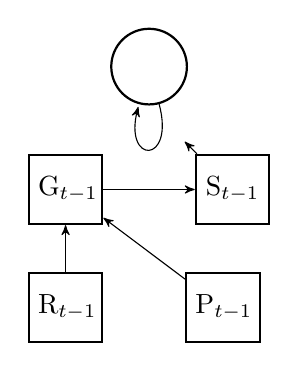
\begin{tikzpicture}[->,>=stealth',auto,thin]
\tikzstyle{every state}=[shape=rectangle,draw,thick,text=black, text centered, text width=0.7cm, align=center]

\node[state]		(A) [shape=circle]             {};
\node[state]        (B) [below of=A, node distance=0.5cm,draw=none] {};
\node[state]		(C) [below left of=B,node distance=1.5cm] {G$_{t-1}$};
\node[state]		(D) [below of=C,node distance=1.5cm] {R$_{t-1}$};
\node[state]        (E) [right of=D,node distance=2cm] {P$_{t-1}$};
\node[state]		(F) [below right of=B,node distance=1.5cm] {S$_{t-1}$};

\path
(A) edge[loop below] (A)
(C) edge (F)
(D) edge (C)
(E) edge (C)
(F) edge (B);
\end{tikzpicture}
\caption{}
\label{fig:subfig2}
\end{subfigure}
\begin{subfigure}[b]{0.3\textwidth}
    \centering
    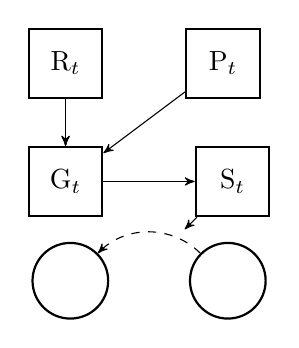
\begin{tikzpicture}[->,>=stealth',auto,thin]
\tikzstyle{every state}=[shape=rectangle,draw,thick,text=black, text centered, text width=0.7cm, align=center]

\node[state]		(A) [shape=circle]             {};
\node[state]        (B) [right of=A, node distance=2cm,shape=circle] {};
\node[state]        (C) [right of=A, node distance=1cm,draw=none] {};
\node[state]        (D) [above of=C, node distance=0.2cm,draw=none] {};
\node[state]		(E) [above left of=D,node distance=1.5cm] {G$_{t}$};
\node[state]		(F) [above of=E,node distance=1.5cm] {R$_{t}$};
\node[state]        (G) [right of=F,node distance=2cm] {P$_{t}$};
\node[state]		(H) [above right of=D,node distance=1.5cm] {S$_{t}$};

\path
(B) edge[dashed,bend left=-45] (A)
(E) edge (H)
(F) edge (E)
(F) edge (E)
(G) edge (E)
(H) edge (D)
;
\end{tikzpicture}
\caption{}
\label{fig:subfig3}
\end{subfigure}
\begin{subfigure}[b]{0.3\textwidth}
    \centering
    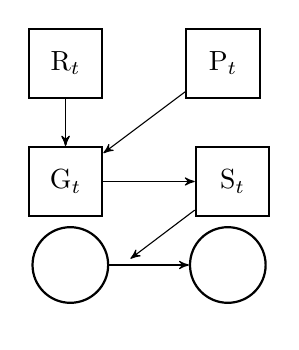
\begin{tikzpicture}[->,>=stealth',auto,thin]
\tikzstyle{every state}=[shape=rectangle,draw,thick,text=black, text centered, text width=0.7cm, align=center]

\node[state]		(A) [shape=circle]             {};
\node[state]        (B) [right of=A, node distance=2cm,shape=circle] {};
\node[state]        (C) [right of=A, node distance=1cm,draw=none] {};
\node[state]        (D) [below right of=A, node distance=0.4cm,draw=none] {};
\node[state]		(E) [above left of=C,node distance=1.5cm] {G$_{t}$};
\node[state]		(F) [above of=E,node distance=1.5cm] {R$_{t}$};
\node[state]        (G) [right of=F,node distance=2cm] {P$_{t}$};
\node[state]		(H) [above right of=C,node distance=1.5cm] {S$_{t}$};

\path
(A) edge (B)
(E) edge (H)
(F) edge (E)
(F) edge (E)
(G) edge (E)
(H) edge (D)
;
\end{tikzpicture}
\caption{}
\label{fig:subfig4}
\end{subfigure}

\caption{Graphical representation of the female human life cycle (a) and the influence of resource dynamics in survival (b) and reproductive (c) dynamics. The female human life cycle (a) is represented with a life cycle graph, dividing the life cycle in four stages: J as the sexually immature stage (i.e. juvenile), A as the sexually mature but without descendants stage (i.e. adult), RC as the stage where individuals reproduce (i.e. reproductive career), and PR as the stage where individuals no longer can reproduce (i.e. post-reproductive). The influence of resource dynamics in survival (b) is based on the amount of resources stored from the last iteration (S$_{t-1}$), which depend on the amount of resources produced (P$_{t-1}$), received (R$_{t-1}$), and gave away (G$_{t-1}$) in the last iteration. The influence of resource dynamics in reproduction (c) is based on the amount of resources stored in the current iteration (S$_t$), which depend on the amount of resources produced (P$_{t}$), received (R$_{t}$), and gave away (G$_{t}$) in that iteration. The influence of resource dynamics in the transition of life cycle stages (d) is based on the amount of resources stored in the current iteration (S$_t$), which depend on the amount of resources produced (P$_{t}$), received (R$_{t}$), and gave away (G$_{t}$) in that iteration. Loop arrows below life cycle stages refers to the probability of staying in that stage (i.e. survival). A newborn is produced either when an individual transition from stage A to RC or when an individual remains in stage RC. The dashed arrows refers to the production of a descendant in that life cycle (i.e. reproduction). The thick arrows between life cycle stages refers to the transition from one stage to the other. The thick arrows between resource dynamics refers to the relationship among them, and which one is used to evaluate survival, reproduction, and life cycle stage transition}.
    \label{fig:1}
\end{figure}

\clearpage

\bibliographystyle{apalike}
\bibliography{optimal_ref}

\end{document}
